\documentclass[tikz,border=0pt]{standalone}
\usepackage[utf8]{inputenc}
\usepackage[T1]{fontenc}
\usepackage{lmodern}
\usepackage{amsmath,amssymb}
\usetikzlibrary{arrows.meta,positioning,fit,calc,backgrounds,shapes.geometric,decorations.pathreplacing}
\definecolor{navy}{HTML}{163A5F}
\definecolor{blue}{HTML}{2C6EAF}
\definecolor{lightblue}{HTML}{EAF2F8}
\definecolor{midblue}{HTML}{CFE1F2}
\definecolor{graytext}{HTML}{4A5560}
\definecolor{lightgray}{HTML}{F4F6F8}
\definecolor{green}{HTML}{3C8D73}
\definecolor{lightgreen}{HTML}{E8F5EF}
\definecolor{red}{HTML}{B24A4A}
\definecolor{lightred}{HTML}{FBEDEE}
\tikzset{
  title/.style={font=\sffamily\bfseries\fontsize{18}{20}\selectfont,text=navy,anchor=west},
  subtitle/.style={font=\sffamily\bfseries\fontsize{11}{13}\selectfont,text=navy},
  body/.style={font=\sffamily\fontsize{9.2}{11}\selectfont,text=graytext,align=left},
  small/.style={font=\sffamily\fontsize{8}{9.4}\selectfont,text=graytext,align=left},
  tinylabel/.style={font=\sffamily\fontsize{7.2}{8.4}\selectfont,text=graytext},
  panel/.style={rounded corners=3pt,draw=midblue,fill=white,line width=0.6pt},
  box/.style={rounded corners=2pt,draw=midblue,fill=lightblue,line width=0.6pt},
  worker/.style={rounded corners=2pt,draw=blue,dashed,line width=0.7pt,fill=white},
  task/.style={rounded corners=2pt,draw=blue,fill=lightblue,minimum width=0.85cm,minimum height=0.55cm,font=\sffamily\bfseries\small,text=navy},
  file/.style={draw=blue,fill=white,minimum width=0.55cm,minimum height=0.42cm,font=\sffamily\small,text=navy},
  arr/.style={-{Stealth[length=2.4mm,width=1.8mm]},draw=blue,line width=0.9pt},
  arrthin/.style={-{Stealth[length=2mm,width=1.5mm]},draw=blue,line width=0.7pt},
  arrred/.style={-{Stealth[length=2mm,width=1.5mm]},draw=red,dashed,line width=0.8pt},
  arrgreen/.style={-{Stealth[length=2mm,width=1.5mm]},draw=green,dotted,line width=1pt}
}
\begin{document}

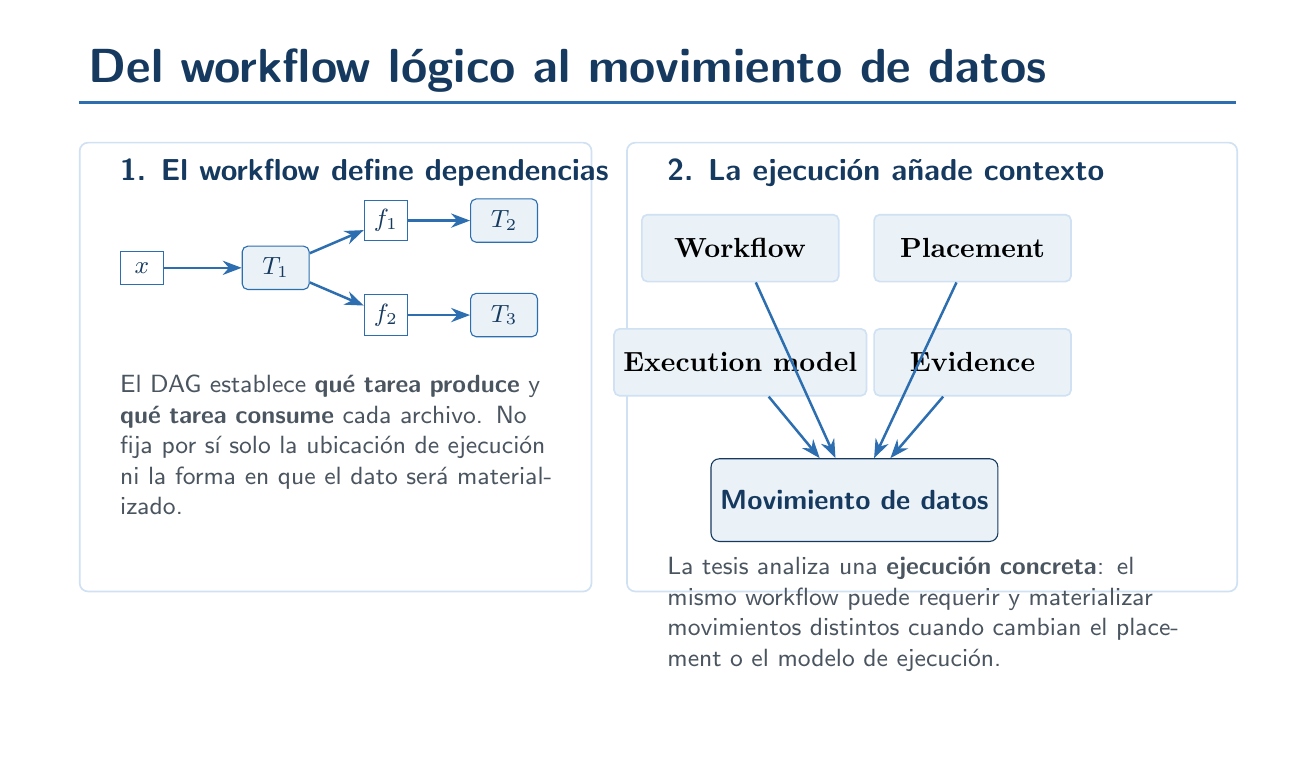
\begin{tikzpicture}[x=1cm,y=1cm]
\path[use as bounding box] (0,0) rectangle (16,9);
\node[title] at (0.65,8.45) {Del workflow lógico al movimiento de datos};
\draw[blue,line width=1pt] (0.65,8.05)--(15.35,8.05);

\node[panel,minimum width=6.5cm,minimum height=5.7cm,anchor=north west] (p1) at (0.65,7.55) {};
\node[subtitle,anchor=west] at (1.05,7.15) {1. El workflow define dependencias};
\node[file] (in) at (1.45,5.95) {$x$};
\node[task] (t1) at (3.15,5.95) {$T_1$};
\node[file] (f1) at (4.55,6.55) {$f_1$};
\node[file] (f2) at (4.55,5.35) {$f_2$};
\node[task] (t2) at (6.05,6.55) {$T_2$};
\node[task] (t3) at (6.05,5.35) {$T_3$};
\draw[arr] (in)--(t1);
\draw[arr] (t1)--(f1); \draw[arr] (f1)--(t2);
\draw[arr] (t1)--(f2); \draw[arr] (f2)--(t3);
\node[body,text width=5.55cm] at (3.95,3.7) {El DAG establece \textbf{qué tarea produce} y \textbf{qué tarea consume} cada archivo. No fija por sí solo la ubicación de ejecución ni la forma en que el dato será materializado.};

\node[panel,minimum width=7.75cm,minimum height=5.7cm,anchor=north west] (p2) at (7.6,7.55) {};
\node[subtitle,anchor=west] at (8.0,7.15) {2. La ejecución añade contexto};
\node[box,minimum width=2.5cm,minimum height=0.85cm] (wf) at (9.05,6.2) {\textbf{Workflow}};
\node[box,minimum width=2.5cm,minimum height=0.85cm] (pl) at (12.0,6.2) {\textbf{Placement}};
\node[box,minimum width=2.5cm,minimum height=0.85cm] (em) at (9.05,4.75) {\textbf{Execution model}};
\node[box,minimum width=2.5cm,minimum height=0.85cm] (tr) at (12.0,4.75) {\textbf{Evidence}};
\node[rounded corners=3pt,draw=navy,fill=lightblue,minimum width=3.2cm,minimum height=1.05cm,font=\sffamily\bfseries,text=navy] (dm) at (10.5,3.0) {Movimiento de datos};
\draw[arr] (wf)--(dm); \draw[arr] (pl)--(dm); \draw[arr] (em)--(dm); \draw[arr] (tr)--(dm);
\node[body,text width=6.65cm] at (11.45,1.55) {La tesis analiza una \textbf{ejecución concreta}: el mismo workflow puede requerir y materializar movimientos distintos cuando cambian el placement o el modelo de ejecución.};
\end{tikzpicture}
\end{document}
